\subsection{Синтез управляющего устройства СПС третьего порядка без учета нелинейности}
Выполним синтез СПС для  управляемого объекта третьего порядка с дифференциальными уравнениями, описывающими систему  \eqref{eq:con_sys_VSS}.
\begin{equation}
    \left\{
    \begin{aligned} \label{eq:con_sys_VSS}
       p\,\left(81\,p^2+108\,p+1\right)\,x&=-3\,u&&, \text{ если}|u|\le 0.6\\
       p\,\left(81\,p^2+108\,p+1\right)\,x&=-1.8\,\mathrm{sign}\left(u\right)&&, \text{ если}|u|> 0.6\\
    \end{aligned}
    \right.
\end{equation}

Было установлено, что, система должна иметь замкнутую структуру, при этом в силу специфики объекта для обеспечения качественного управления эта структура должна быть переменной. На первом этапе аналитического конструирования не будем учитывать характер входных воздействий и ограничения вида насыщения, а синтезируем систему, обеспечивающую качественные показатели в свободном движении, причиной которых являются начальные возмущения - отклонения от какого-либо равновесного состояния. Основными требованиями к системе будем считать точность, характер переходного процесса, быстродействие. Конкретные значения этих показателей уточним в процессе синтеза системы.
Отсюда математическое описание системы в виде переменных состояния при $u\le0.6$ \eqref{eq:ss_object_VSS}.
\begin{equation}\label{eq:ss_object_VSS}    \left\{    \begin{aligned}x_1&=x , \\ \cfrac{d\,x_1}{d\,t}&=x_2 ,\\ \cfrac{d\,x_2}{d\,t}&=x_3,\\\cfrac{d\,x_3}{d\,t}&=-
0.0123
\,x_2-
1.3333
\,x_3-
0.0370
\,u    \end{aligned}    \right.\end{equation}

     Рассмотрим возможность положительного решения задачи синтеза при простейшей структуре СПС со скользящим движением, а именно, синтезируем СПС с управлением вида:
\begin{equation} \label{eq:}
u=\psi\,x_1
\end{equation}
\begin{equation}\label{eq:}
\psi=
    \left\{
    \begin{aligned}
&\alpha &&,\text{ если } x_1\,S>0 \\
&\beta &&,\text{ если } x_1\,S<0 \\
    \end{aligned}
    \right.
\end{equation}

Где $\alpha,\beta$ --- постоянные коэффициенты. 
 $S=x_3+c_2\,x_2+c_1\,x_1$ --- уравнение, задающее некоторую гиперплоскость, которая является при принятых выше соотношениях границей разрыва управляющего воздействия $u$.
	Так как фактически структура системы определена, в результате синтеза необходимо определить параметры СПС, а именно, значения $\beta,\alpha,c_1,c_2$, обеспечивающие требуемые показатели качества разрабатываемой системы. 
Отсюда приведенный ХП замкнутой системы :
\begin{equation} \label{eq:}
D(p)=\,p^3+1.333\,p^2+0.01235\,p+0.03704\,\psi
\end{equation}
\begin{equation} \label{eq:}
a_3=1.333,a_2=0.01235,a_1=0,b=0.03704
\end{equation}

Итак должны соблюдаться 3 условия:
\begin{enumerate}
\item 
Условия существования  скользящего режима для системы 3-ого порядка  имеют вид:
\begin{equation}
    \begin{aligned} \label{eq:}
       b\,\alpha&>c_1\,(a_3-c_2)\\
       b\,\beta&<c_1\,(a_3-c_2)\\
       \cfrac{c_1-a_2}{c_2}&=c_2-a_3\\
    \end{aligned}
\end{equation}
Или эквивалентная форма:
\begin{equation}
    \begin{aligned} \label{eq:}
       &\alpha>f(c_2)>\beta\\
       &\text{Где } f(c_2)=e_1\,c_2^3+e_2\,c_2^2+e_3\,c_2+e_4\\
       &e_1=-\cfrac{1}{b}, e_2=\cfrac{2\,a_3}{b}, e_3=\cfrac{-(a_3^2+a_2)}{b}, e_4=\cfrac{a_2\,a_3}{b}\\
       &e_1=-27, e_2=72, e_3=-48.3, e_4=0.444\\
    \end{aligned}
\end{equation}
\item 
Условие обеспечения устойчивости движения в скользящем режиме: ХП системы  \eqref{eq:HP_VSS} должен иметь не более 1-ого корня с положительной вещественной частью. Формулировка имеет вид  \eqref{eq:VSS_steady}.
\begin{equation}
    \begin{aligned} \label{eq:HP_VSS}
       D(p)&=\,p^3+a_3\,p^2+a_2\,p+b\,\psi=\\
       &=\,p^3+1.333\,p^2+0.01235\,p+0.03704\,\psi\\
       \psi&=\cfrac{-c_1(c_2-a_3)}{b}\\
    \end{aligned}
\end{equation}
\begin{equation} \label{eq:VSS_steady}
Re(p_i)>0 \text{ только для одного } i\in(1,2,3)
\end{equation}
\item
Условия для попадания изображающей точки на плоскость скольжения --- в ХП  \eqref{eq:HP1_VSS} неотрицательные действительные корни отсутствуют, т.е. отсутствуют экспоненты с положительной степенью. Формулировка имеет вид  \eqref{eq:VSS_hit_the_plane}.
\begin{equation} \label{eq:HP1_VSS}
D(p)=\,p^3+1.333\,p^2+0.01235\,p+0.03704\,\alpha
\end{equation}
\begin{equation} \label{eq:VSS_hit_the_plane}
\forall i=\overline{1,3}:\left(p_i=Re(p_i)\text{ и }Re(p_i)\ge0\right) \text{ --- не выполняются.}
\end{equation}
\end{enumerate}

Алгоритм расчёта праметров в m-file matlab:
\begin{verbatim}
%% начальные условия------------change
T=InitialConditions.T;
K=InitialConditions.K;
h=InitialConditions.h;
d=InitialConditions.d;

syms p Psi ;
u=Psi ;
disp('        (T^2*p^2+2*h*T*p+1)+K*u ');
D=(T^2*p^3+2*h*T*p^2+p)+K*u ;
disp('           D/(T^2)');
D=collect(D,p);
D=D/(T^2);
D=collect(D,p);
vpa(D,3)
Dp=coeffs(D,p);

a=double([0 Dp(2) Dp(3)]);
b=double(Dp(1)/Psi)
e=[-1 2*a(3) -(a(3)^2+a(2)) a(2)*a(3) ]/b ;

% выбор праметров 
max_inter=10; %---количество итераций максимальное
mn=[2,0.5];%change множитель у alpha и  betta соотв.
near=0;
far=1; %------------------------начало интервалов
step=1; %-------------------------длинна интервала
iter=1;
IT=0;
n=2;
find=1;
tic;

while ((n>1)||(IT==0))
fprintf('\r%s',['итерация номер ',num2str(iter)]);
%выбор C1
near=far;
far=far+step;
%выбор случайного числа из интервала
inter=[near far];
C2=rand*(inter(2)-inter(1))+inter(1);
%---------------------------------
C1=C2^2-a(3)*C2+a(2);
if ~(sign(C1)+1)
iter=iter+1;
continue
end
f=e(1)*C2^3+e(2)*C2^2+e(3)*C2+e(4);
alpha=f+abs(mn(1)*f);
betta=f-abs(mn(2)*f);
%проверка устойчивости
psiv=(-C1*(C2-a(3)))/b;
D1=subs(D,Psi,psiv);
pv=double(solve(D1,p));
n=0;
for i=1:length(pv)
if real(pv(i))>0
n=n+1;
end
end
%---------------------------
%проверка попадания изображающей точки 
%на плоскость скольжения
psiv=alpha;
D1=subs(D,Psi,psiv);
pv=double(solve(D1,p));
IT=1;

for i=1:length(pv)
if pv(i)==real(pv(i))
if real(pv(i))>=0
IT=0;
end
end
end
%----------------------------
if iter>max_inter, find=0; break,else, find=1; end
iter=iter+1;
end

%непонятная вещь, которую необходимо сделать,
% чтобы получить скольжение
C2=C2*3;

\end{verbatim}


В результате расчёта имеем устойчивое движение в скользящем режиме с попаданием изображающей точки на плоскость скольжения.Запустим алгоритм несколько раз с разными параметрами расчёта:

Расчёт номер:1


  Итераций $= 1 [ C_1=1.13 ; C_2=5.75 ; \alpha=17.7 ; \beta=-53.2 ]$

  Время на выполнение программы $1$ сек.

Расчёт номер:2


  Итераций $= 1 [ C_1=0.835 ; C_2=5.38 ; \alpha=10.3 ; \beta=-31 ]$

  Время на выполнение программы $1$ сек.

Расчёт номер:3


  Итераций $= 1 [ C_1=1.24 ; C_2=5.88 ; \alpha=21 ; \beta=-62.9 ]$

  Время на выполнение программы $1$ сек.

Расчёт номер:4


  Итераций $= 1 [ C_1=0.546 ; C_2=4.97 ; \alpha=4.75 ; \beta=-14.3 ]$

  Время на выполнение программы $1$ сек.

Модель в Matlab Simulink на рис.\ref{fig:sim_VSS_P}. 
\begin{figure}[!h]\centering
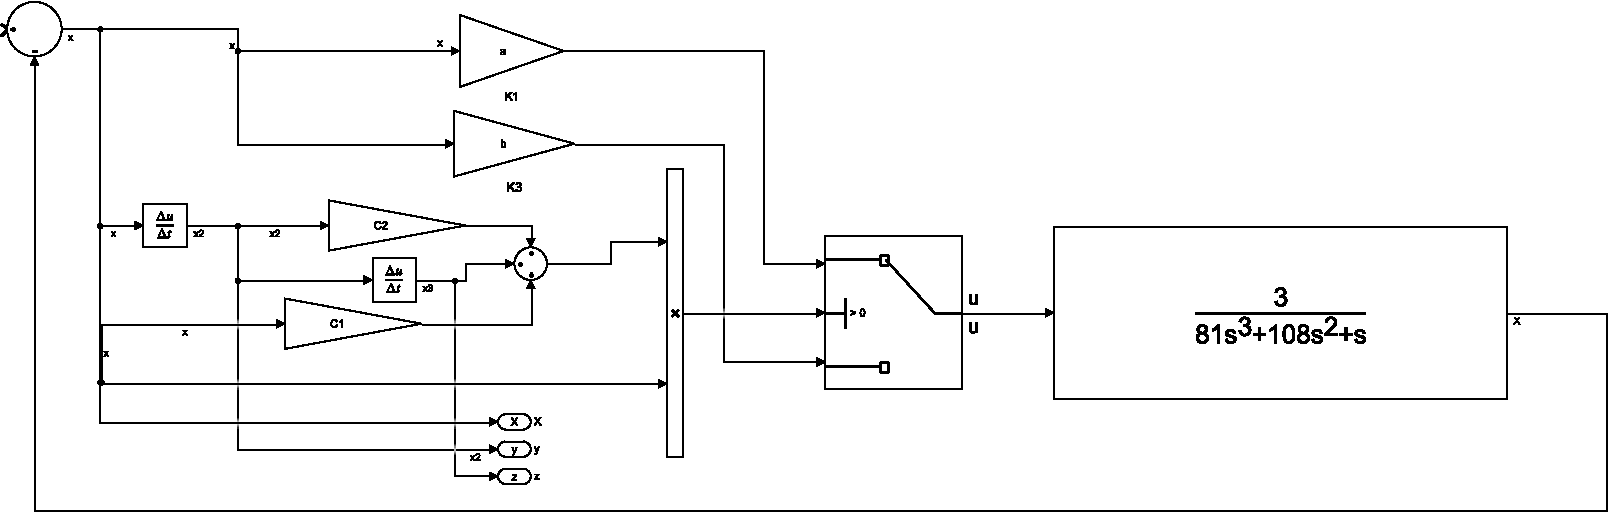
\includegraphics[width=1.0\linewidth]{images/sim_VSS_P}
\caption{Структурная схема СПС 3 порядка со скользящим режимом.}\label{fig:sim_VSS_P}
\end{figure}
Исследуем движение фазовых координат во времени посредством моделирования процессов в системе при отклонении системы от состояния равновесия. Фазовые траектории в системе на рис.\ref{fig:VSS_P_ft_VSS_P_2}. 
В дополнение на рис.\ref{fig:VSS_P_sv_VSS_P} указано изменение выходной переменной и её производной.
В табл.\ref{tab:tab_VSS_3} отобразим время регулирования при разных значениях параметров

\begin{table}[!h] \centering
    \caption{Сравнение результатов} \label{tab:tab_VSS_3}
    \begin{tabular}{|c|c|c|c|c|}
        \hline
        $C_1$ & $C_2$ & $\alpha$ & $\beta$ & $t_p$ \\ \hline
         $1.13$ & $5.75$ & $17.7$ & $-53.2$ & $14$ \\ \hline
         $0.835$ & $5.38$ & $10.3$ & $-31$ & $16.1$ \\ \hline
         $1.24$ & $5.88$ & $21$ & $-62.9$ & $13.4$ \\ \hline
         $0.546$ & $4.97$ & $4.75$ & $-14.3$ & $18.2$ \\ \hline
    \end{tabular}
\end{table}
\begin{figure}[!h]\centering
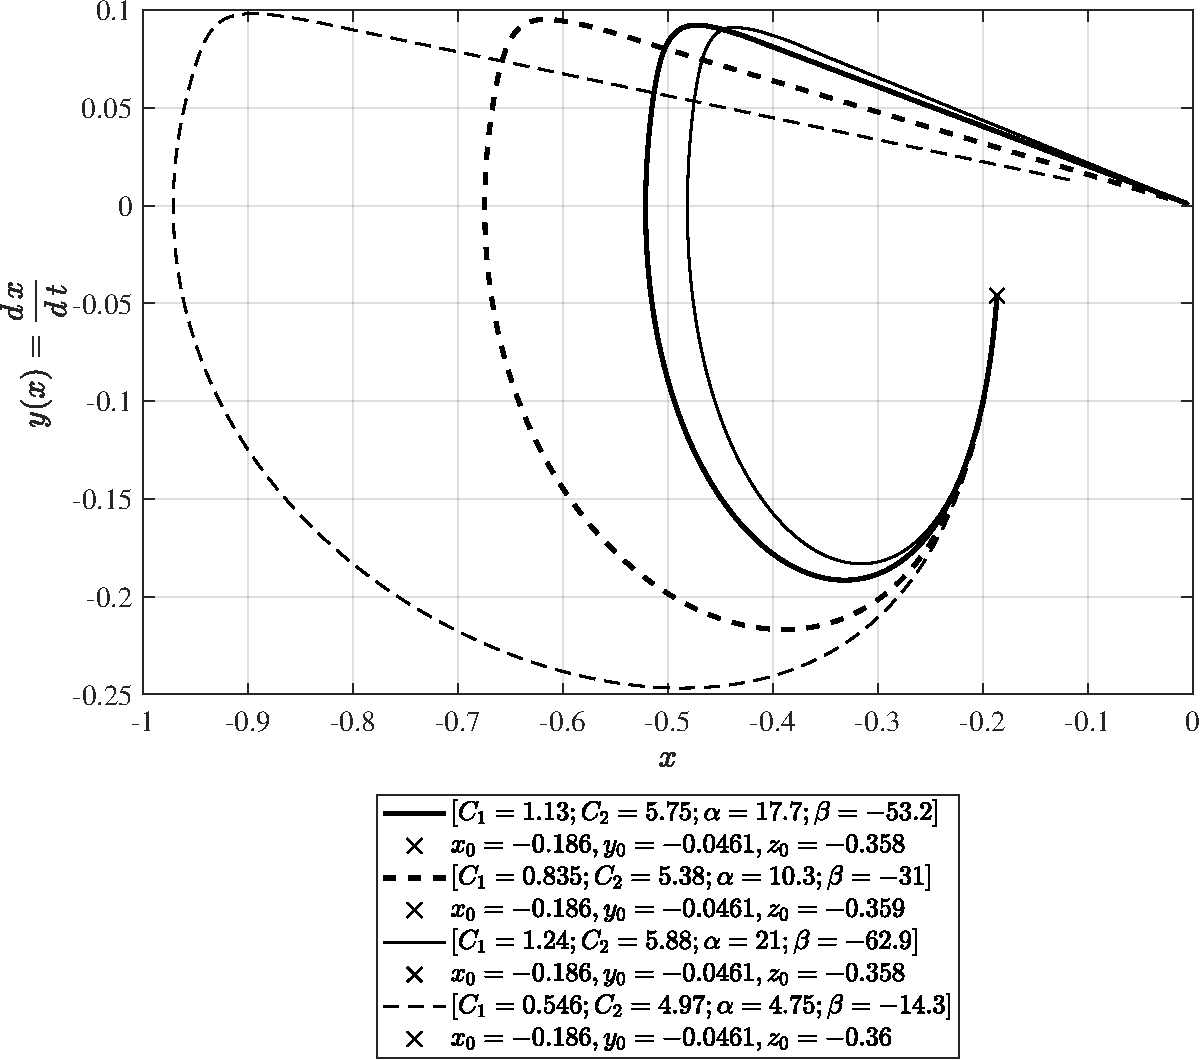
\includegraphics[width=1.0\linewidth]{images/VSS_P_ft_VSS_P_2}
\caption{ Фазовые траектории для системы с переменной структурой для переменных состояния $x_1,x_2$.}\label{fig:VSS_P_ft_VSS_P_2}
\end{figure}
\begin{figure}[!h]\centering
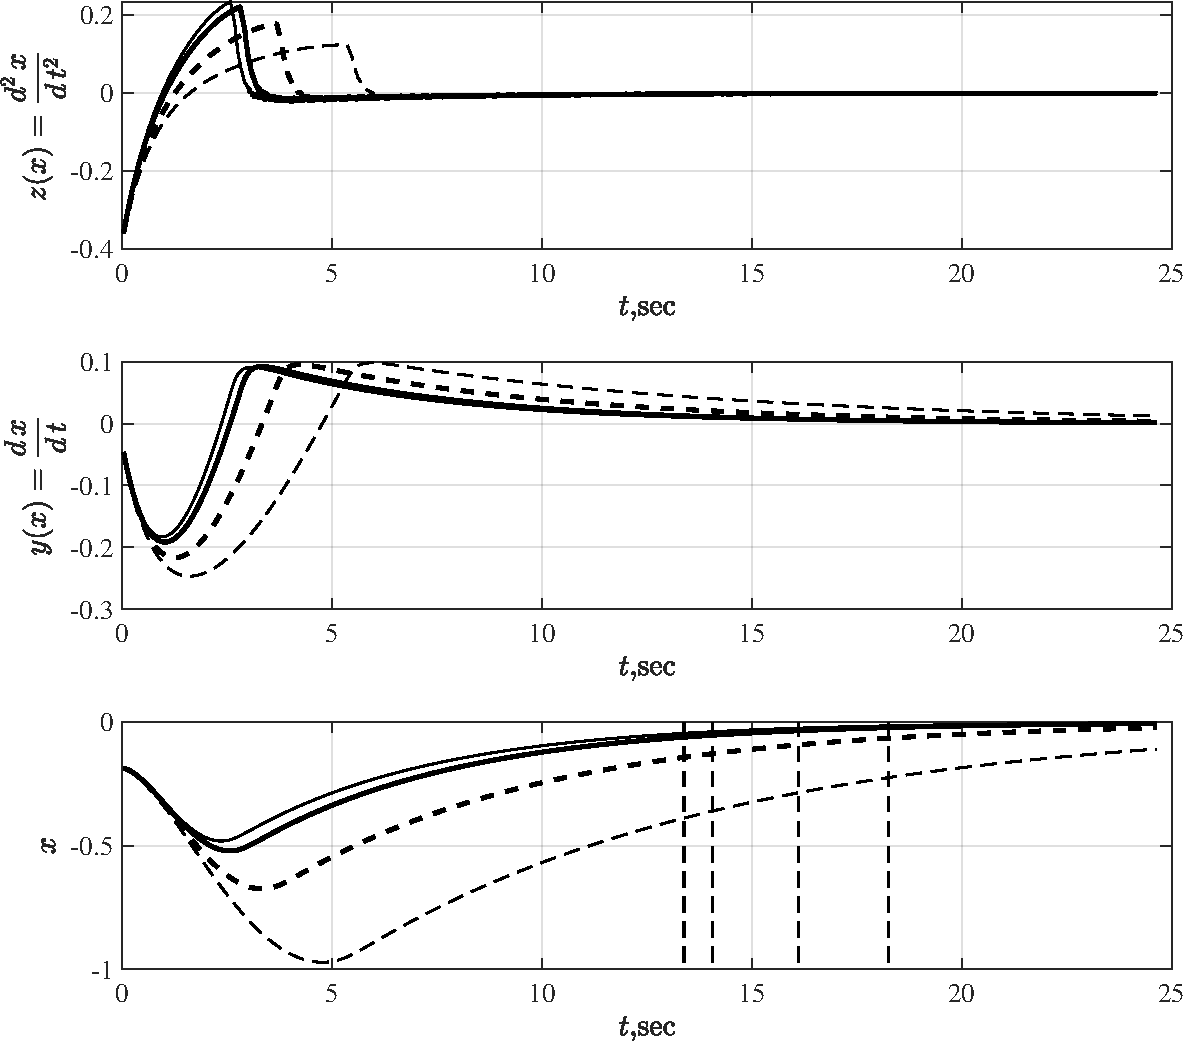
\includegraphics[width=1.0\linewidth]{images/VSS_P_sv_VSS_P}
\caption{ Графики изменения переменных состояния.}\label{fig:VSS_P_sv_VSS_P}
\end{figure}


Полученные характеристики позволяют сравнить качественные показатели СПС и обычной линейной системы. Из переходных характеристик СПС следует, что переходный процесс имеет апериодический характер, при этом время переходного процесса меньше, чем в линейной системе. Изменяя параметры СПС, можно влиять на качественные показатели системы. Однако для таких изменений необходимо определить пределы изменения параметров, руководствуясь условиями устойчивости и условиями попадания изображающей точки на плоскость скольжения.
Чем больше $\alpha$, тем быстрее заканчивается переходный процесс,

Определим запас устойчивости системы <<в малом>> по амплитуде и фазе, построив логарифмические частотные характеристики для разомкнутой системы с $\alpha=21$ на рис.\ref{fig:Bode_diagram_alpha} и $\beta=-62.9$ на рис.\ref{fig:Bode_diagram_beta}. 
\begin{equation} \label{eq:}
W=\cfrac{3\,\psi}{p\,\left(81\,p^2+108\,p+1\right)}
\end{equation}
\begin{figure}[!h]\centering
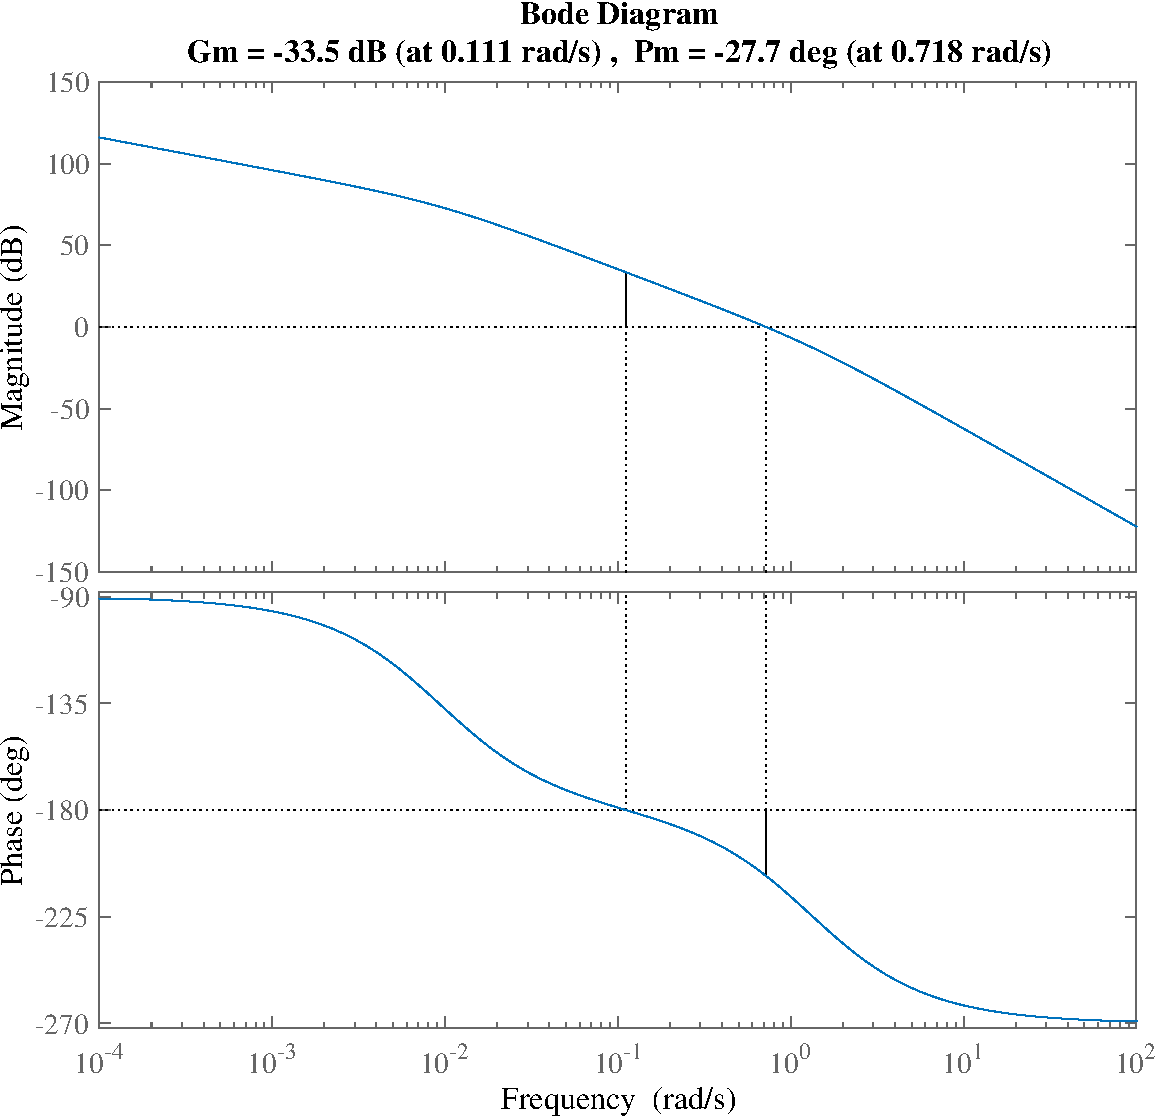
\includegraphics[width=1.0\linewidth]{images/Bode_diagram_alpha}
\caption{ Логарифмические частотные характеристики разомкнутой системы с $\alpha$}\label{fig:Bode_diagram_alpha}
\end{figure}
\begin{figure}[!h]\centering
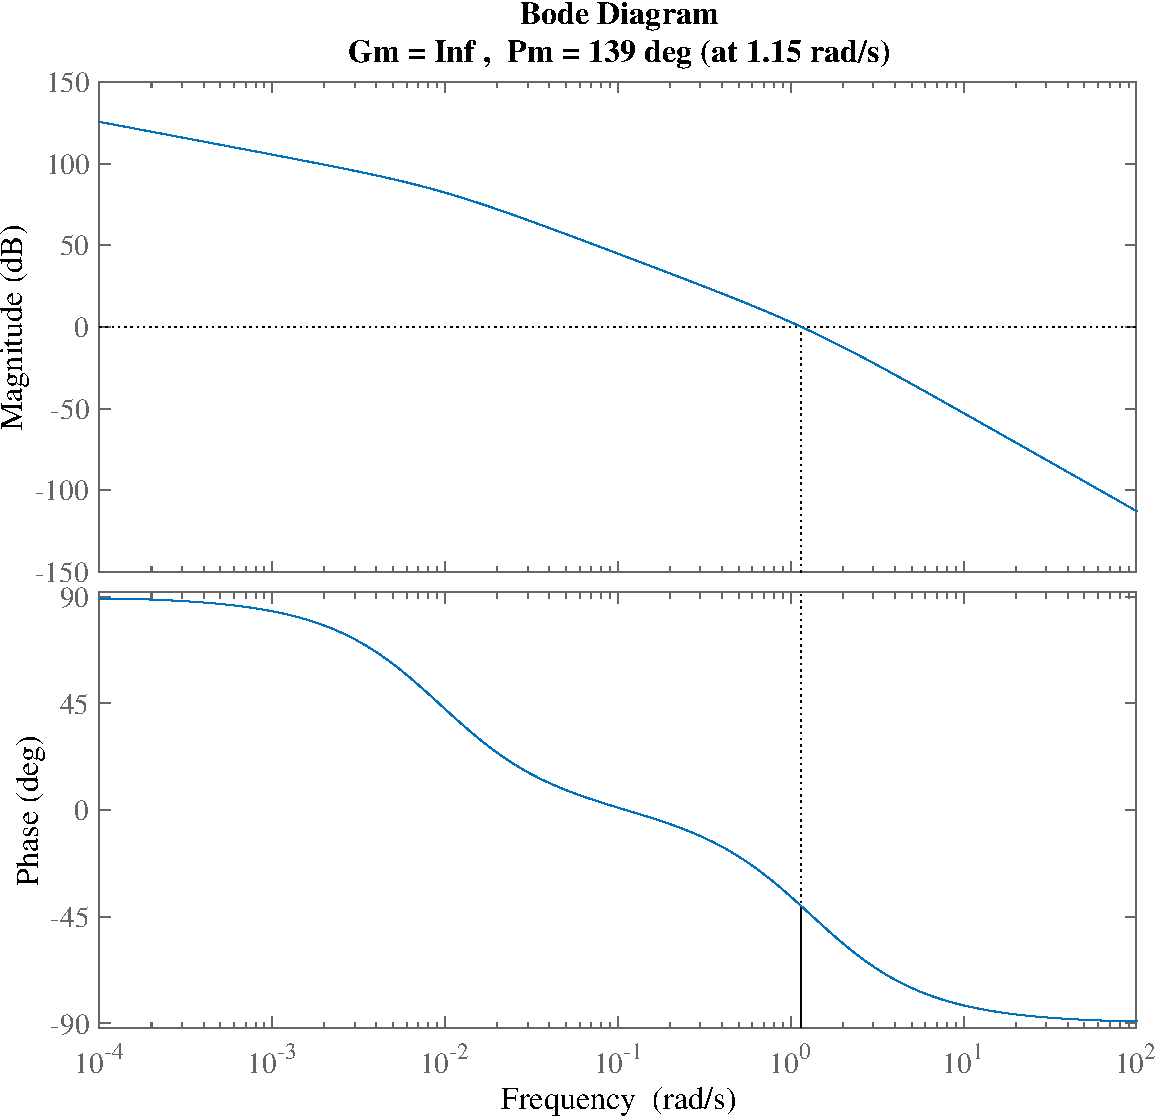
\includegraphics[width=1.0\linewidth]{images/Bode_diagram_beta}
\caption{ Логарифмические частотные характеристики разомкнутой системы с $\beta$}\label{fig:Bode_diagram_beta}
\end{figure}
Таким образом, в результате синтеза СПС со скользящим режимом без учета нелинейного элемента мы получили систему, обладающую характеристиками, соответствующими техническому заданию, а именно:
\begin{enumerate}
\item 
Для $\alpha$ запас устойчивости <<в малом>> по амплитуде $-33.5<$ 20 дБ, по фазе $-27.7< 60°$, $\omega_{cp}=0.718$. 
\item 
Для $\beta$ запас устойчивости <<в малом>> по амплитуде $Inf\ge$ 20 дБ, по фазе $139\ge 60°$, $\omega_{cp}=1.15$. 
\end{enumerate}
